\subsection{Comparación de densidades} \label{cap:densidades}

Una vez que se tuvo seguridad con los sensores elegidos se procedió a realizar una placa con estos elementos para que no se desconecten y no se produzcan errores como solía suceder mientras estaban en la protoboard (Figura \ref{fig:sensoresa}). \\
\begin{figure}[H]
	\centering
	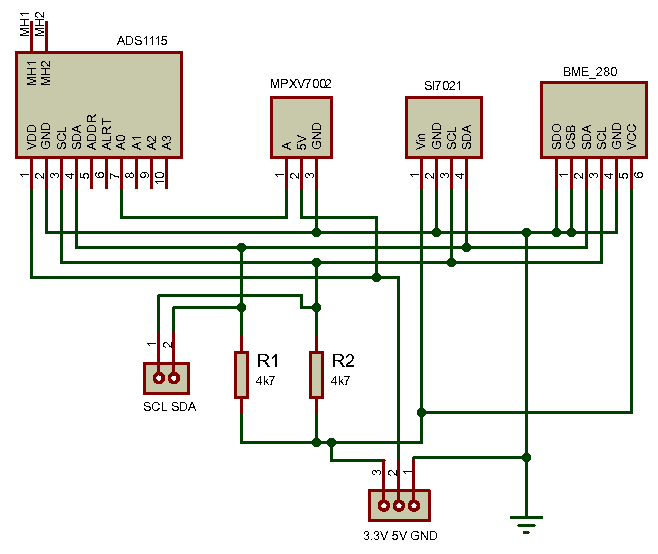
\includegraphics[scale=0.8]{placa_sensores.pdf}
	\captionof{figure}{Esquema de placa con sensores utilizados}
	\label{fig:sensoresa}
\end{figure}

A raíz de varias mediciones, durante distintos días, y realizando el contraste con el instrumento \textbf{TESTO 435} se decidió sacar de la caja donde estaban a los sensores de temperatura y humedad para que luego el cálculo de la velocidad del aire no esté desfasado, ya que esta caja utilizada generaba un ambiente distinto al real dentro del laboratorio. Al colocar el sensor del lado externo, se realizaron tomas de valores en distintos momentos. Con ambos conjuntos de datos se procedió a obtener los valores de la densidad calculados con la fórmula. Estos datos están expresados en la tabla \ref{densicalc}. 


\begin{table}[b]
	\centering
	\begin{tabular}{ll|l|l|l|l|l|l|l|l|l|}
		\cline{3-11}
		\multicolumn{2}{c}{} & \multicolumn{2}{|c|}{\textbf{T [$^{\circ}$$C$]}} & \multicolumn{2}{c|}{\textbf{H [$\%$] }} & \multicolumn{2}{c|}{\textbf{P [$Pa$]}} &  \multicolumn{2}{c|}{\textbf{\begin{tabular}[c]{@{}c@{}}Dens. calculada\\ {[}$kg/m^3${]}\end{tabular}}} & \multicolumn{1}{c|}{\multirow{2}{*}{\textbf{$e_r$ [$\%$]}}} \\ \cline{1-10}
		\multicolumn{1}{|c|}{\textbf{Fecha}} & \multicolumn{1}{c|}{\textbf{Obs.}} & \multicolumn{1}{c|}{\textbf{I}} & \multicolumn{1}{c|}{\textbf{S}} & \multicolumn{1}{c|}{\textbf{I}} & \multicolumn{1}{c|}{\textbf{S}} & \multicolumn{1}{c|}{\textbf{I}} & \multicolumn{1}{c|}{\textbf{S}} & \multicolumn{1}{c|}{\textbf{I}} & \multicolumn{1}{c|}{\textbf{S}} & \multicolumn{1}{c|}{} \\ \hline
		\multicolumn{1}{|l|}{29-abr} & interior & 19,4 & 19,3 & 43,5 & 38,5 & 100400 & 100450 & 1,1916 & 1,1931 & 0,128 \\ \hline
		\multicolumn{1}{|l|}{14-may} & interior & 16,1 & 18,4 & 54,6 & 43,5 & 101590 & 101570 & 1,2195 & 1,2099 & 0,781 \\ \hline
		\multicolumn{1}{|l|}{14-may} & interior & 16,5 & 18,9 & 53,7 & 42,5 & 101559 & 101559 & 1,2173 & 1,2077 & 0,794 \\ \hline
		\multicolumn{1}{|l|}{17-jun} & exterior & 15,2 & 15,5 & 54,3 & 48,6 & 103100 & 103090 & 1,2418 & 1,2404 & 0,109 \\ \hline
		\multicolumn{1}{|l|}{17-jun} & exterior & 13,8 & 15,1 & 59,2 & 52,4 & 102970 & 102910 & 1,2463 & 1,2397 & 0,527 \\ \hline
		\multicolumn{1}{|l|}{07-jul} & interior & 17,6 & 18,8 & 43,3 & 34,8 & 100260 & 100261 & 1,1978 & 1,1933 & 0,375 \\ \hline
	\end{tabular}
	\caption{Comparación de densidades calculadas}
	\label{densicalc}
\end{table}




Referencias de la tabla:
\begin{itemize}
	\item \textbf{I}: Instrumentos- Datos obtenidos con los instrumentos del Laboratorio de fluidos.
	\item \textbf{S}: Sensores- Datos obtenidos a partir de la medición con los sensores utilizados en conjunto con Arduino.
	\item \textbf{interior}- Mientras se realizaron las mediciones el sensor SH21 se encontraba dentro de la caja dónde estaba el Arduino y la placa reguladora.
	\item \textbf{exterior}- Las mediciones se realizaron con el sensor SH21 en el lado exterior sin que fuera afectado por el calentamiento del Arduino y la placa reguladora.
\end{itemize}


Tomando como valor verdadero los valores de THP medidos con los instrumentos calibrados, se puede observar que el error relativo es menor al 1\%.

\subsection{Fluctuaciones de velocidad}
A partir de la teoría que se observó en la sección \ref{sec:flujoT} figura \ref{fig:fluct}, se decidió corroborar esta propiedad, se utilizó datos medidos y a través de un código generado en Matlab y se constató que el promedio de las fluctuaciones que tiende a cero (Figura \ref{fig:fluct2}).
\begin{figure}[H]
	\centering
	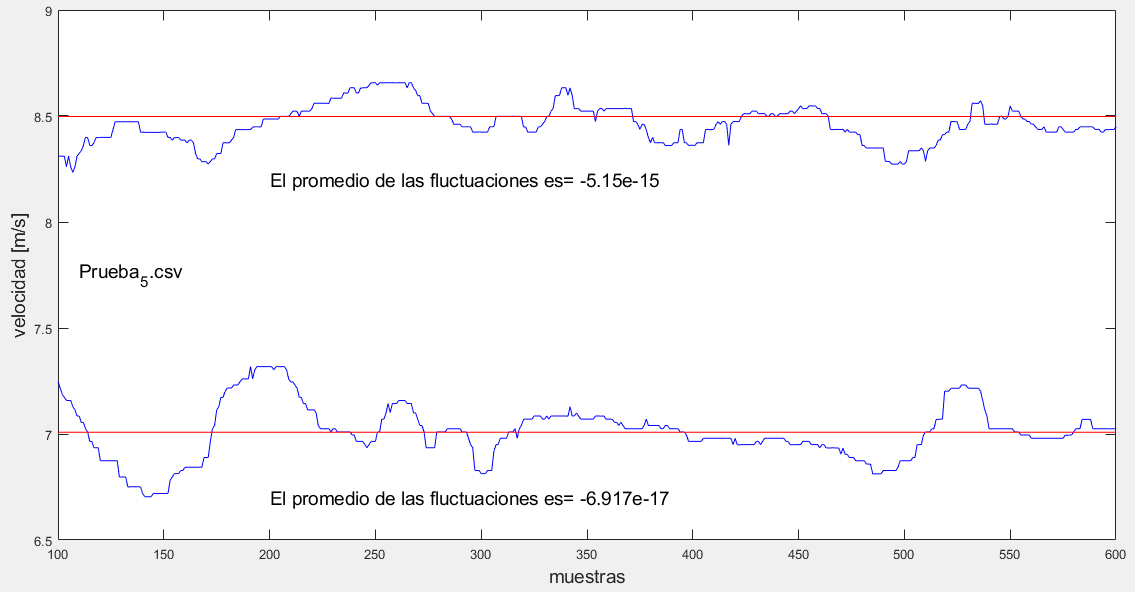
\includegraphics[scale=0.5]{fluctua.png}
	\captionof{figure}{Fluctuaciones en velocidades medidas}
	\label{fig:fluct2}
\end{figure}

%C:\Users\glori\Desktop\DANIELA\VISUAL_DANI\Proyecto_Final_Tunel\Pruebas22.03.21

\subsection{Estimación de la densidad ante cambios de Temperatura y Humedad}
Notamos conveniente realizar la comparación de las densidades calculadas ante las variaciones que se tenían de humedad y temperatura respecto a los datos tomados por los elementos calibrados. En la tabla \ref{densTH} se observa en las celdas internas los valores calculados de densidad para humedad de 38$\%$ y 40$\%$ y temperatura 19$^{\circ}$C y 21$^{\circ}$C, estos datos fueron elegidos al observar las máximas variaciones de los datos tomados con el sensor \textit{SH21} y el instrumento \textit{Testo 435}, manteniendo presión atmosférica constante.
(Los valores con fondo gris corresponden a la diferencia de valores)

\begin{table}[h!]
	\centering
	\begin{tabular}{lllll}
		&  & \multicolumn{2}{c}{\textbf{Temperatura}} &  \\
		&  & \multicolumn{1}{c}{\textbf{19°C}} & \multicolumn{1}{c}{\textbf{21°C}} & \multicolumn{1}{c}{\textbf{}} \\
		\multicolumn{1}{c}{} & \multicolumn{1}{r}{\textbf{38\%}} & 1,1945758 & 1,1859383 & \cellcolor[HTML]{F2F2F2}-0,0086376 \\
		\multicolumn{1}{c}{\multirow{-2}{*}{\textbf{Humedad}}} & \multicolumn{1}{r}{\textbf{40\%}} & 1,1943783 & 1,1857162 & \cellcolor[HTML]{F2F2F2}-0,0086621 \\
		& \multicolumn{1}{c}{\textbf{}} & \cellcolor[HTML]{F2F2F2}-0,0001976 & \cellcolor[HTML]{F2F2F2}-0,0002221 & 
	\end{tabular}
\caption{Densidad del aire ante cambios de TH}
\label{densTH}
\end{table}

Si se calcula la velocidad del aire con la formula \ref{ec_aire} y con los datos de la tabla \ref{densTH} utilizando una diferencia de presión constante de 32$Pa$ se puede observar que la diferencias de velocidades son inferiores a 0,03m/s (tabla \ref{velTH}) ante un cambio de dos grados de temperatura por lo que no se ve necesario realizar una corrección de valores.
(Los valores con fondo gris corresponden a la diferencia de valores)
\begin{table}[h!]
	\centering
	\begin{tabular}{lllll}
		&  & \multicolumn{2}{c}{\textbf{Temperatura}} &  \\
		&  & \multicolumn{1}{c}{\textbf{19°C}} & \multicolumn{1}{c}{\textbf{21°C}} & \multicolumn{1}{c}{\textbf{}} \\
		\multicolumn{1}{c}{} & \multicolumn{1}{r}{\textbf{38\%}} & 7,3195288 & 7,3461357 & \cellcolor[HTML]{F2F2F2}0,0266068 \\
		\multicolumn{1}{c}{\multirow{-2}{*}{\textbf{Humedad}}} & \multicolumn{1}{r}{\textbf{40\%}} & 7,3201342 & 7,3468236 & \cellcolor[HTML]{F2F2F2}0,0266894 \\
		& \multicolumn{1}{c}{\textbf{}} & \cellcolor[HTML]{F2F2F2}0,0006054 & \cellcolor[HTML]{F2F2F2}0,0006879 & 
	\end{tabular}
\caption{del aire ante cambios de TH}
\label{velTH}
\end{table}

\subsection{comparación de la frecuencia vista en el panel con el valor de PWM}
\subsection{Contrastación de diferencia de presión}

El sensor \textit{MPX7002} tiene como salida voltaje proporcional a la diferencia de presión medida, por lo que fue necesario utilizar un \textit{ASD1115} para transformar estos valores, a través de una constante, en unidades de presión.

Para realizar la contrastación de la diferencia de presión ocasionada dentro del túnel por el aire, se procedió a realizar mediciones con el instrumento calibrado \textit{AXD 650}. Al poseer fluctuaciones anteriormente habladas a causa del flujo turbulento, se procedió a filmar el instrumento y aparte los datos obtenidos por nuestro sistema. Ambos videos se unieron y se realizaron diversas pausas para tomar al mismo tiempo ambos valores leídos. Como resultado se obtuvo la tabla \ref{difpres}, generando luego un gráfico de puntos con las muestras tomadas, observando que el error es mayor para diferencias de presión mayores a 100 Pa \ref{fig:condifpres}.

\begin{figure}[H]
	\centering
	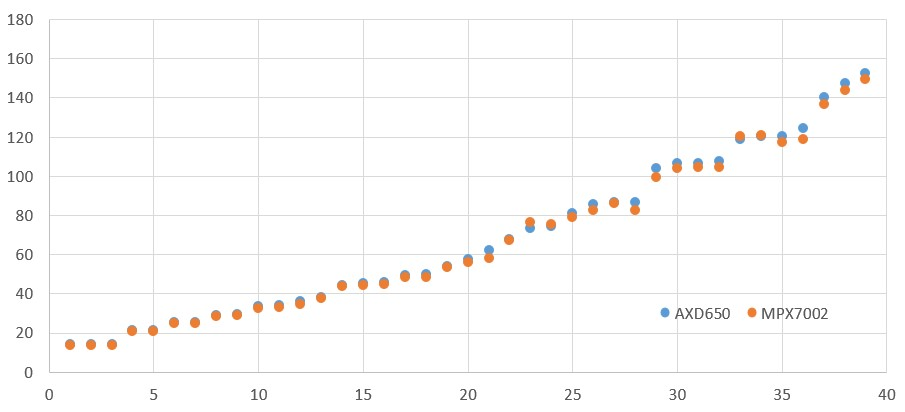
\includegraphics[scale=0.5]{condifpres.jpg}
	\captionof{figure}{Contrastación de diferencia de presión}
	\label{fig:condifpres}
\end{figure}

\begin{table}[h!]%diferencia de presion
		\centering
		\begin{tabular}{|r|r|r}
			\cline{1-2}
			\multicolumn{2}{|c|}{Diferencia de presión {[}Pa{]}} & \multicolumn{1}{c}{} \\ \hline
			\multicolumn{1}{|c|}{\textbf{AXD650}} & \multicolumn{1}{c|}{\textbf{MPX7002}} & \multicolumn{1}{c|}{\textbf{E$_r$}} \\ \hline
			14 & 13,51 & \multicolumn{1}{r|}{3,50\%} \\ \hline
			14 & 13,76 & \multicolumn{1}{r|}{1,71\%} \\ \hline
			14 & 13,76 & \multicolumn{1}{r|}{1,71\%} \\ \hline
			21,3 & 20,88 & \multicolumn{1}{r|}{1,97\%} \\ \hline
			21,5 & 20,88 & \multicolumn{1}{r|}{2,88\%} \\ \hline
			25,3 & 24,8 & \multicolumn{1}{r|}{1,98\%} \\ \hline
			25,4 & 24,8 & \multicolumn{1}{r|}{2,36\%} \\ \hline
			28,9 & 28,51 & \multicolumn{1}{r|}{1,35\%} \\ \hline
			29,3 & 28,8 & \multicolumn{1}{r|}{1,71\%} \\ \hline
			33,4 & 32,5 & \multicolumn{1}{r|}{2,69\%} \\ \hline
			34,1 & 32,88 & \multicolumn{1}{r|}{3,58\%} \\ \hline
			35,9 & 34,8 & \multicolumn{1}{r|}{3,06\%} \\ \hline
			38,1 & 37,38 & \multicolumn{1}{r|}{1,89\%} \\ \hline
			44,2 & 43,88 & \multicolumn{1}{r|}{0,72\%} \\ \hline
			45,5 & 44,5 & \multicolumn{1}{r|}{2,20\%} \\ \hline
			45,9 & 44,88 & \multicolumn{1}{r|}{2,22\%} \\ \hline
			49,4 & 48,51 & \multicolumn{1}{r|}{1,80\%} \\ \hline
			49,9 & 48,51 & \multicolumn{1}{r|}{2,79\%} \\ \hline
			54 & 53,26 & \multicolumn{1}{r|}{1,37\%} \\ \hline
			57,7 & 56,2 & \multicolumn{1}{r|}{2,60\%} \\ \hline
			62,1 & 58,13 & \multicolumn{1}{r|}{6,39\%} \\ \hline
			68 & 67,13 & \multicolumn{1}{r|}{1,28\%} \\ \hline
			73,4 & 76,6 & \multicolumn{1}{r|}{-4,36\%} \\ \hline
			74,3 & 75,26 & \multicolumn{1}{r|}{-1,29\%} \\ \hline
			81,1 & 79,01 & \multicolumn{1}{r|}{2,58\%} \\ \hline
			85,5 & 82,76 & \multicolumn{1}{r|}{3,20\%} \\ \hline
			86,4 & 86,1 & \multicolumn{1}{r|}{0,35\%} \\ \hline
			86,8 & 82,63 & \multicolumn{1}{r|}{4,80\%} \\ \hline
			104 & 99,26 & \multicolumn{1}{r|}{4,56\%} \\ \hline
			106,5 & 104,13 & \multicolumn{1}{r|}{2,23\%} \\ \hline
			106,8 & 104,5 & \multicolumn{1}{r|}{2,15\%} \\ \hline
			107,8 & 104,63 & \multicolumn{1}{r|}{2,94\%} \\ \hline
			118,8 & 120,13 & \multicolumn{1}{r|}{-1,12\%} \\ \hline
			120,4 & 120,6 & \multicolumn{1}{r|}{-0,17\%} \\ \hline
			120,5 & 117,38 & \multicolumn{1}{r|}{2,59\%} \\ \hline
			124,4 & 119 & \multicolumn{1}{r|}{4,34\%} \\ \hline
			140,1 & 136,6 & \multicolumn{1}{r|}{2,50\%} \\ \hline
			147,2 & 143,8 & \multicolumn{1}{r|}{2,31\%} \\ \hline
			152,7 & 149,38 & \multicolumn{1}{r|}{2,17\%} \\ \hline
		\end{tabular}
	\caption{Comparación de Diferencia de presión}
	\label{difpres}

\end{table}

\subsection{Contrastación de velocidades}
como contrastación final....
ver PRUEBA\_10\_PID
el error es mucho mayor que el de velocidad en funcion de la TH. no tiene sentido comparar ambos porq para ellos usamos  un anemómetro (podriamos ver de usar el anemómetro de ventilador? y el de testo para ver los distintos valores y nosotros con el código en función de THP)





